\documentclass[a4paper]{article}

\usepackage[english]{babel}
\usepackage[utf8x]{inputenc}
\usepackage{amsmath}
\usepackage{graphicx}
\usepackage[colorinlistoftodos]{todonotes}
\usepackage{color}
\usepackage{hyperref}
\usepackage{fullpage}
\usepackage{titling}
\usepackage{float}

\newcommand{\subtitle}[1]{%
  \posttitle{%
    \par\end{center}
    \begin{center}\large\end{center}}
}

\title{\textbf{Open Information Systems\\Assignment part 3}}
\subtitle{2015-2016 Vrije Universiteit Brussel\\Responsible tutor : Christophe Debruyne - chrdebru@vub.ac.be}
\author{\textbf{Team Trackerspace}\\Matteo Marra - mmarra@vub.ac.be - 0525999 - 1M Comp Sci Soft\\Antoine Carpentier - antcarpe@vub.ac.be - 0529527 - 1M Comp Sci AI\\Titouan Christophe - tichrist@vub.ac.be - 0529190 - 1M Comp Sci Soft\\Bruno Rocha Pereira - brochape@vub.ac.be - 0529512 - 1M Comp Sci Soft}

\begin{document}

\maketitle

\section{Abstract}
\section{Introduction}

Our application will help users to share and rate their favorite locations and tracks for exercises of all sorts. Users will interact in three ways : 

\begin{enumerate}
    \item Record and share tracks (where they run, bike...)
    \item Tag those tracks with specific keywords for other users to discover them
    \item Record and share spots where they exercise along tracks
\end{enumerate}

The following document describes the process of the development of a ontology common with all the other groups. It includes the difficulties we encountered during this process and the changes that were applied to our model in order to achieve a better interoperability.


\todo{Check if more is needed}


\section{Elaboration of the ontology}
Due to the high number of students that had to take part in the realisation of the main ontology, a meeting on Slack\footnote{https://ontology-ois.slack.com} was organized. The first meeting there led, after a challenging discussion, to the first and only definition present in the ontology common to food and exercise : "A calorie is a unit of energy, it is gained by eating and lost during physical activity. A calorie equals 4.184 Joules." 

After the main ontology was defined, we all decided to split into two groups. The first group was composed of the four groups working on the \textit{exercise ontology}. The second one was working on the \textit{food ontology}. Both groups discussed their ontologies on separate channels on Slack, namely \texttt{\#exercise} and \texttt{\#food}.

Regarding the exercise group, we immediately started working on common definitions such as \textit{workout}. It was decided after a short discussion that it would be more suitable for each group to first define every one of the terms appearing in their application.  Therefore, every group shared a glossary and a diagram of their model. Another meeting was scheduled two days later to merge and adapt the definitions that would later appear in the \textit{exercise ontology}. 
During this meeting, at least one member of each group was present on the Slack channel to avoid any bias. It was implicitely decided not to have every member of each group connected in order to avoid confusion and overlapping discussions. 
We decided to proceed concept by concept, starting from a definition of \texttt{Exercise} and its properties (such as \texttt{Heart Rate}, \texttt{Equipment}, \texttt{Duration}, \texttt{Difficulty}, \texttt{Rating}, \texttt{Muscle Group}, \texttt{Repetition}).
In order to link the exercises with the global ontology, we decided to put the number of calories burned as property of an \texttt{Exercise}.

\texttt{Workout} was then defined to link an exercise session, composed by many \texttt{Exercise}, user and date.
The last concept defined during that meeting was \texttt{User} as the account of the user using the application.
At the end of the meeting, all the common entities were decided and defined.

The last meeting happened five days later in one of the computer rooms. Two members of each group were present and the ontology was ported to Webprotégé \footnote{http://starpc14.vub.ac.be:8080/webprotege/\#Edit:projectId=0f54f43f-f27d-46f0-a5bc-de5e7574ab98}. 
This operation has been done from a unique computer in order to avoid concurrency problems, with all members present to the meeting participating to this process.
In this meeting we decided that some concept we defined would refer to an already existing ontology, namely \texttt{Person}\footnote{http://dbpedia.org/ontology/Person} and \texttt{Muscle group}\footnote{http://dbpedia.org/page/Category:Muscles\_by\_location}.

Later on, during the lab session, it was decided to change \texttt{User} to \texttt{UserAccount}, linking it with a \texttt{ownedBy} property to \texttt{Person}.

The ontology was then checked via the OOPS platform and the group 3 took care of correcting all of the warnings. 

\subsection{Difficulties}
The first difficulty all the groups encountered appeared while searching for the common definition for "Calorie". It was difficult to synchronize different opinions and ideas with so much people and it took several hours to reach a common definition everybody agreed with.

We did not encounter the same kind of difficulties for the \textit{exercise ontology}, since it was a much smaller group and we easily agreed on the definition of the common entities.
In this phase the main difficulty our group encountered was that our application is significantly different from all the others, since the main purpose of it is storing track records, and not gym exercises like most of the others do.
We decided that, in order to have a more suitable ontology for all the groups, it was better to slightly change our model, adding some supplementary functionalities that would anyway not change the purpose of our application. 
We agreed to add to the ontology the concepts of \texttt{Workout} and \texttt{Heart\_Rate} that were not included in our model but were easy to integrate. \todo{check my english please}
Our entity \texttt{Exercise\_Spot} wasn't present in any of the other groups, and together with the other groups we decided to add the concept \texttt{Equipment} in the ontology.

We did not encounter any problem in the inter-group communication. 

\subsection{Changes to the model}
We made a few minor changes to our model in order to fit the agreed ontology. These changes have no impact on our application purpose and scope.

\subsubsection{Add a Workout entity}
The elaborated ontology specifies a workout entity, which model a user that performs a sport session. We therefore added a \texttt{Workout} to our database, which refers to tracks a user has run and the exercices he made during a workout session. This is simply a wrapper for our specialized activity types.

\subsubsection{Exercise session}
The informations we recorded for exercices spot in our database only included the user rating. We therefore added the \texttt{Exercise\_Session} entity, which models the fact that a user perform a certain number of \textbf{repetitions} of an exercise at an exercise spot, along with its \textbf{heart rate} during the session, in order to comply with the workout ontology. The exercise session is an implementation for the exercise spots of our \texttt{Record} entity (which was for tracks).



\begin{figure}[h!]
  \center
  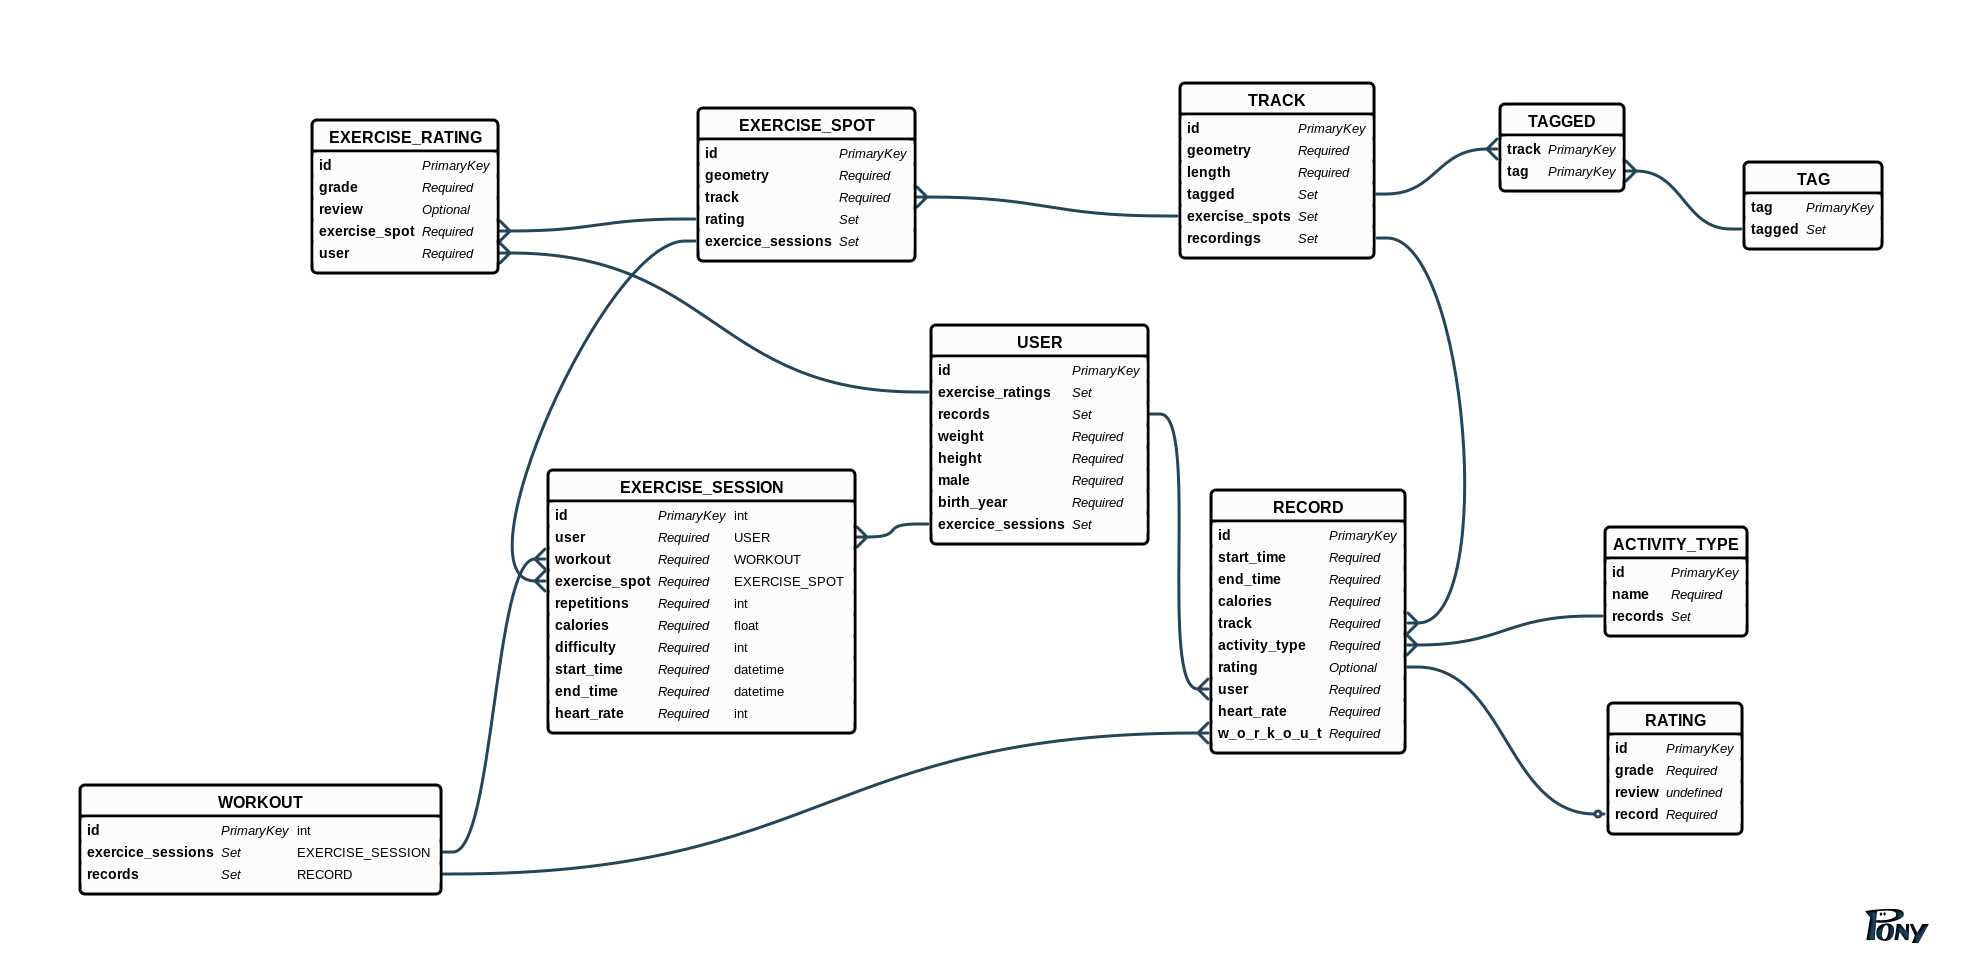
\includegraphics[width=\textwidth]{er.png}
  \caption{\label{fig:new-er} The updated Entity/Relationship diagram of our model}
\end{figure}

\begin{figure}[h!]
  \center
  \includegraphics[width=\textwidth]{er-old.png}
  \caption{\label{fig:old-er} The previous version of our Entity/Relationship diagram, for comparison with Figure \ref{fig:new-er}}
\end{figure}


%Add workout
%Heart rate?
%exercise record (it's just another 'implementation' of exercise defined in the ontology (along with record)
%These changes were applied in order to fit the ontology and were suitable add-ons to our application. No change that would make the application loose its main purpose were made.
%Say that workout is just a wrapper for exercises/traks.
%%NEW ER DIAGRAM
\subsection{Contributions}
Bruno Rocha Pereira and Matteo Marra participated to the ontology meetings after consulting with the rest of the group and reporting in group meetings which were the choice made. 
Titouan Christophe and Antoine Carpentier took care of defining our new model and applying the changes we needed. 
\section{Conclusion}


\end{document}
